
\documentclass[10 pt,usenames,dvipsnames, oneside]{article}
\usepackage{../../modelo-fracoes}
\graphicspath{{../../../Figuras/licao03/}}


\begin{document}

\begin{center}
  \begin{minipage}[l]{3cm}

\includegraphics[width=2cm]{../../../Figuras/logo}       
\end{minipage}\hfill
\begin{minipage}[r]{.8\textwidth}
 {\Large \scshape Atividade: Varal dos números}  
\end{minipage}
\end{center}
\vspace{.2cm}

\ifdefined\prof
%Caixa do Para o Professor
\begin{goals}
%Objetivos específicos
\begin{enumerate}
\item Representar frações na reta numérica. 
\item Ordenar frações na reta numérica.
\end{enumerate}

\tcblower

%Orientações e sugestões
\noindent {\bf Material necessário:}
\begin{itemize} %s
  \item     Barbante suficiente para cobrir a extensão de uma das paredes da sala de aula (por exemplo, aquela em que está posicionado o quadro).
  \item  Folhas de papel (para confeccionar os cartões numerados).
  \item  32 prendedores para fixar os cartões no barbante (podem ser pregadores de roupa, clipes ou mesmo fita adesiva).
  \item     Fita adesiva ou equivalente (para fixar o barbante na parede).
\end{itemize} %s

\noindent {\bf Preparação para a atividade:}
\begin{itemize} %s
  \item     Esta atividade deve ser desenvolvida como um jogo, envolvendo todos os alunos da turma, organizados em grupos com 5 ou 6 alunos. Tudo deve ser combinado e esclarecido antes de a atividade começar.
  \item  O professor deve fazer um  ``varal'' com o barbante em um local que seja visível para todos os alunos e não muito alto para que os estudantes possam alcançar com as mãos. Esse barbante representará a reta numérica.
  \item A proposta da atividade é ``pendurar os números'' no barbante usando pregadores ou fitas adesivas, visando experimentar, em uma atividade concreta, a associação entre os pontos da reta e os números. Para isso, serão feitos cartões numerados.
  \item É importante reforçar a fixação das extremidades do barbante para que não solte com o peso dos cartões que serão pendurados.
  \item Use o papel para produzir os cartões numerados. Garanta que o tamanho dos números permita a visualização por todos os alunos. 
  \item  Números a serem escritos nos cartões numerados: $0$, $1$, $2$, $3$, $\frac{1}{2}$, $\frac{2}{2}$, $\frac{3}{2}$, $\frac{4}{2}$, $\frac{5}{2}$, $\frac{6}{2}$, $\frac{1}{3}$, $\frac{2}{3}$, $\frac{3}{3}$, $\frac{4}{3}$, $\frac{7}{3}$, $\frac{9}{3}$, $\frac{1}{4}$, $\frac{2}{4}$, $\frac{3}{4}$, $\frac{4}{4}$, $\frac{5}{4}$, $\frac{6}{4}$, $\frac{8}{4}$, $\frac{10}{4}$, $\frac{11}{4}$, $\frac{12}{4}$, $\frac{1}{5}$, $\frac{3}{5}$, $\frac{4}{5}$, $\frac{6}{5}$, $\frac{7}{5}$, $\frac{10}{5}$, $\frac{1}{10}$.
  \item Garanta que haja pelo menos um cartão numerado para cada aluno. Se necessário, amplie a quantidade de cartões numerados. A sequência com 32 números é básica. 
\end{itemize} %s

\textbf{Discussões sobre o desenvolvimento da atividade}
\begin{itemize}
  \item O desenvolvimento da atividade precisa ser mediado pelo professor. O processo e a discussão são importantes.
  \item Os cartões com o 0 (zero) e como 1 (um) devem ser presos no barbante pelo professor antes do início da atividade. A distância entre o 0 (zero) e o 1 (um) identifica a unidade, que determinará a marcação dos demais números.
  \item Garanta que haja espaço no barbante  para a fixação de todos os cartões numerados. Considerando a sequência de 32 cartões, observe que há 9 números entre o zero e o um e o maior número a ser fixado é o 3.
  \item Recomenda-se que, para facilitar a comunicação, os grupos sejam identificados, por exemplo, por cores. Cada grupo, na sua vez de jogar, deve fixar um cartão numerado no varal e outro grupo deve avaliar se o cartão foi fixado em uma posição correta ou não.
  \item Distribua os cartões igualmente entre os grupos.
  \item A correção da fixação realizada por um grupo pode ser decidida por outro grupo, devendo ser discutida com toda a turma.
  \item Pontuação: cada cartão numerado posicionado corretamente vale um ponto para o grupo que fixou o cartão. Cada avaliação correta vale meio ponto para o grupo que ficou responsável por ela.
  \item Vence o jogo o grupo que, após a fixação de todos os cartões numerados no varal, tiver acumulado maior quantidade de pontos.
  \item Em cada rodada, todos os grupos devem prender um cartão numerado no varal e avaliar a colocação feita por outro grupo. Varie as duplas de grupos que farão as ações de fixação/avaliação de cada cartão preso no varal. Assim, por exemplo, se a turma estiver organizada em $5$ grupos (azul, verde, vermelho, amarelo e preto), com 6 alunos cada um, na primeira rodada as duplas que farão a fixação/avaliação podem ser, por exemplo, azul/preto, verde/vermelho, vermelho/azul, amarelo/verde e preto/amarelo. Já na segunda rodada as duplas podem ser azul/amarelo, verde/preto, vermelho/verde, amarelo/azul e preto/vermelho. Planeje previamente essas associações e comunique aos alunos para não gerar discussão durante a realização. Uma forma de determinar as duplas dos grupos é o sorteio. 
  \item Incentive e procure fazer, respeitando as questões pessoais, com que cada aluno fixe um cartão numerado no varal. 
  \item Escolha o grupo com o cartão de número 2  para dar início ao jogo e, em seguida, aquele que tiver o número 3.  Quando já presos no varal, esses cartões facilitarão a fixação dos demais, em que há números não inteiros.
  \item Observe que alguns cartões numerados ocuparão a mesma posição na reta. Por exemplo, os numerados com $2$ e $\frac{4}{2}$. Nesses casos, recomenda-se que o segundo cartão a ser fixado seja preso no que já está no varal, sem que um esconda o outro. Sugere-se um abaixo do outro. Aproveite esses casos para discutir com os alunos que um mesmo número pode ter mais do que uma representação.
  \item Muito provavelmente as frações de denominador $2$ serão as mais fáceis de serem fixadas no varal. Em seguida, as de denominador $4$. As fixações das frações de denominadores $3$, $5$ e $10$ devem impor um pouco mais de desafio. Garanta que haja equilíbrio de dificuldade na distribuição dos cartões numerados entre os grupos.
  \item Estimule a discussão interna nos grupos para a decisão da posição de fixação de cada cartão numerado. O aluno eleito pelo grupo para prender o cartão no barbante deve explicar como decidiram por aquela posição.
  \end{itemize}

    \textbf{Sugestões de variação do jogo}\newline

\begin{itemize}  
  \item Versão individual: colocam-se os cartões embaralhados sobre a mesa do professor com as faces voltadas para baixo e cada estudante deve pegar um cartão e posicioná-lo no varal.
  \item Outra versão em grupo: pede-se que cada grupo sugira frações para que outro grupo faça a fixação. Nesse caso, as frações podem ser escolhidas a partir de uma lista previamente estabelecida pelo professor. Recomenda-se que o grupo que escolher a fração faça a leitura e que o grupo que fizer a fixação registre simbolicamente essa fração. Dessa forma, a leitura e a escrita em representação simbólica também podem ser tratadas na atividade.
\end{itemize} %s
\end{goals}

\bigskip
\begin{center}
{\large \scshape Atividade}
\end{center}
\fi

O varal de números está disposto na sala de aula, nele já estão posicionados os números $0$ (zero) e $1$ (um), como na figura. Nos cartões preparados para a atividade estão os números: \\
$0$, $1$, $2$, $3$, $\frac{1}{2}$, $\frac{2}{2}$, $\frac{3}{2}$, $\frac{4}{2}$, $\frac{5}{2}$, $\frac{6}{2}$,
$\frac{1}{3}$, $\frac{2}{3}$, $\frac{3}{3}$, $\frac{4}{3}$, $\frac{7}{3}$, $\frac{9}{3}$,
$\frac{1}{4}$, $\frac{2}{4}$, $\frac{3}{4}$, $\frac{4}{4}$, $\frac{5}{4}$, $\frac{6}{4}$, $\frac{8}{4}$, $\frac{10}{4}$, $\frac{11}{4}$, $\frac{12}{4}$,
$\frac{1}{5}$, $\frac{3}{5}$, $\frac{4}{5}$, $\frac{6}{5}$, $\frac{7}{5}$, $\frac{10}{5}$,
$\frac{1}{10}$.

\begin{center}
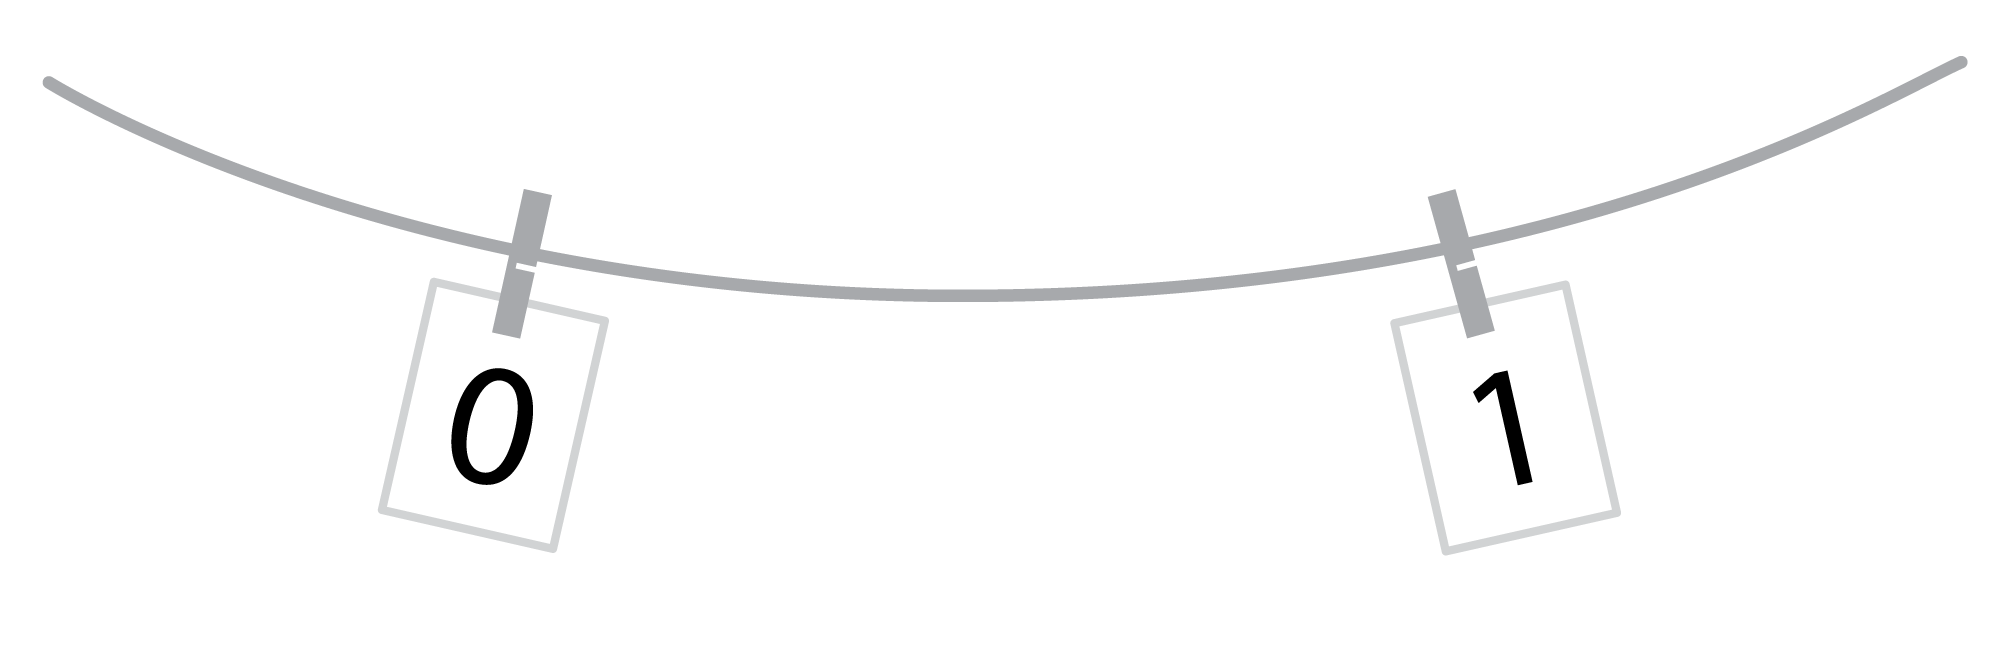
\includegraphics[width=300pt, keepaspectratio]{ativ11_fig01.png}
\end{center}


O jogo consiste em fixar cartões numerados em varal, reproduzindo uma reta numérica. As regras serão apresentadas pelo seu professor ou professora. Discuta com seus colegas a posição correta de fixação de cada um dos cartões numerados no varal.

Ao final do jogo, reproduza a forma como os cartões foram posicionados no varal na reta numérica a seguir. Aproveite as marcações já existentes.

\begin{center}
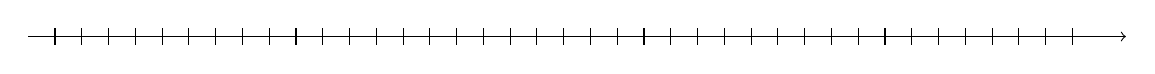
\begin{tikzpicture}[x=34mm,y=34mm]
\draw[->] (-0.1,0) -- (4,0) ; %reta anterior
\foreach \x in {0,.1,...,3.9}{ \draw (\x,3pt) -- (\x,-3pt);}
\end{tikzpicture}
\end{center}

\ifdefined\prof
\begin{solucao}

Para facilitar a visualização a solução é apresentada em duas retas.
  \begin{center}
\begin{tikzpicture}[x=23mm,y=34mm]
  \draw[->] (-0.1,0) -- (3.3,0) ; %reta anterior

\foreach \x in {0,.1,...,3.2}{ \draw (\x,1pt) -- (\x,-1pt);}
\foreach \x in {0,1,2,3}{
  \draw[dashed, thick, lightgray] (\x,0) -- (\x,-.53);
  \node at (\x,-24pt) {\x};
}
\foreach \x in {1,2,3,4,5,6} {
  \fill[attention] (\x/2, 0) circle (1pt);
  \node[above] at (\x/2,0) {$\frac{\x}{2}$};
}
\foreach \x in {1,2,3,4,7,9} {
  \fill[common] (\x/3, 0) circle (1pt);
  \node[below] at (\x/3,0) {$\frac{\x}{3}$};
}
\fill[common] (0,0) circle (1pt);
\fill[common] (0.1,0) circle (1pt);
\node[above] at (0.1,0) {$\frac{1}{10}$};

\begin{scope}[yshift=-50]
\draw[->] (-0.1,0) -- (3.3,0) ; %reta anterior
\foreach \x in {0,.1,...,3.2}{ \draw (\x,1pt) -- (\x,-1pt);}
\foreach \x in {1,2,3,4,5,6,8,10,11,12} {
  \fill[attention] (\x/4, 0) circle (1pt);
  \node[above] at (\x/4,0) {$\frac{\x}{4}$};
}
\foreach \x in {1,3,4,6,7,10} {
  \fill[common] (\x/5, 0) circle (1pt);
  \node[below] at (\x/5,0) {$\frac{\x}{5}$};
}
\fill[common] (0,0) circle (1pt);
\fill[common] (0.1,0) circle (1pt);
\node[above] at (.1,0) {$\frac{1}{10}$};
\end{scope}
\end{tikzpicture}

\end{center}


\end{solucao}
\fi

\end{document}